\section{Price response function implementations}
\label{sec:response_functions_imp}

The main objective of this work is to analyze the price response functions. In
general we define the self- and cross-response functions in a correlated
financial market as
\begin{equation}\label{eq:response_general}
    R^{\left(scale\right)}_{ij}\left(\tau\right)=\left\langle
    r^{\left(scale\right)}_{i}\left(t-1, \tau\right)
    \varepsilon^{\left(scale\right)}_{j} \left(t\right)\right\rangle_{average}
\end{equation}
where the index $i$ and $j$ correspond to stocks in the market,
$r^{\left(scale\right)}_{i}$ is the return of the stock $i$ in a time lag
$\tau$ in the corresponding scale and $\varepsilon^{\left(scale\right)}_{j}$ is
the trade sign of the stock $j$ in the corresponding scale. The superscript
$scale$ refers to the time scale used, whether physical time scale
($scale = p$) or trade time scale ($scale = t$). Finally, The subscript
$average$ refers to the way to average the price response, whether relative to
the physical time scale ($average = P$) or relative to the trade time scale
($average = T$).

We use the returns and the trade signs to define three response functions:
trade time scale response, physical time scale response and activity response.

To compare the three response functions, we define the following quantities
\begin{align}
    E_{j,d}\left(t\right)&=\sum_{n=1}^{N\left(t\right)}
    \varepsilon_{j,d}^{\left(t\right)}\left(t,n\right) =
    \text{sgn}\left(E_{j,d}\left(t\right)\right)
    \left|E_{j,d}\left(t\right)\right|\label{eq:sum_trades}\\
    \varepsilon_{j,d}^{\left(p\right)}\left(t\right)&=
    \text{sgn}\left(E_{j,d}\left(t\right)\right)\label{eq:sign_sum_trades}
\end{align}
where the subscript $d$ refers to the days used in the response computation.
We use Eq. (\ref{eq:sum_trades}) to make easier the comparison between the
results, as all the defined responses use the trade sign term.

In Sect. \ref{subsec:response_function_trade} we analyze the responses
functions in trade time scale, in Sect. \ref{subsec:response_function_physical}
we analyze the responses functions in physical time scale and in Sect.
\ref{subsec:activity_response_function} we define a response function to
analyze the influence of the frequency of trades in a second.

%%%%%%%%%%%%%%%%%%%%%%%%%%%%%%%%%%%%%%%%%%%%%%%%%%%%%%%%%%%%%%%%%%%%%%%%%%%%%%%
\subsection{Response functions on trade time scale}
\label{subsec:response_function_trade}

We define the self- and cross-response functions in trade time scale, using the
trade signs in trade time scale. For the returns, we select the last midpoint
price of every second and compute them. We use this strategy with the TAQ data
set considering that the price response in trade time scale can not be directly
compared with the price response in physical time scale. In this case we relate
each trade sign in one second with the midpoint price of the previous second.
Then, to compute the returns, instead of using trades as the time lag (it would
make no sense as all the midpoint price are the same in one second) we use
seconds. Thus, we force the response in trade time scale to have a physical
time lag, and then, be able to compare with the physical time scale response.
This approximation is feasible considering the discussion in Sect.
\ref{sec:response_functions_def}. The price response function in trade time
scale is defined as
\begin{equation}\label{eq:response_functions_trade_scale_general}
    R^{\left(t\right)}_{ij}\left(\tau\right)=\left\langle r^{\left(p\right)}
    _{i}\left(t-1,\tau \right)\varepsilon_{j}^{\left(t\right)}
    \left(t, n\right)\right\rangle _{T}
\end{equation}
where the superscript $t$ refers to the trade time scale. We explicitly
calculate the average in Eq. (\ref{eq:response_functions_trade_scale_general}),
\begin{align}\label{eq:response_trades_explicit}
    R_{ij}^{\left(t\right)}\left(\tau\right)&=\frac{1}{\sum_{d=d_{0}}^{d_{f}}
    \sum_{t=t_{0}}^{t_{f}}N_{j,d} \left(t \right)} \nonumber \\
    &\sum_{d=d_{0}}^{d_{f}}\sum_{t=t_{0}}^{t_{f}}\sum_{n=1}
    ^{N\left(t\right)} r^{\left(p\right)}_{i,d}\left(t-1, \tau\right)
    \varepsilon_{j,d}^{\left(t\right)}\left(t,n\right)\\
    &=\sum_{d=d_{0}}^{d_{f}}\sum_{t=t_{0}}^{t_{f}} r^{\left(p\right)}_{i,d}
    \left(t-1,\tau\right) \frac{\sum_{n=1}^{N\left(t\right)}
    \varepsilon_{j,d}^{\left(t\right)}\left(t,n \right)}
    {\sum_{d=d_{0}}^{d_{f}} \sum_{t=t_{0}}^{t_{f}}N_{j,d}\left(t\right)}
    \nonumber \\
    &=\sum_{d=d_{0}}^{d_{f}}\sum_{t=t_{0}}^{t_{f}}r^{\left(p\right)}_{i,d}
    \left(t-1,\tau\right) \text{sgn}\left(E_{j,d}\left(t\right)\right)
    w_{j,d}^{\left(t\right)}\left(t\right)
\end{align}
where
\begin{equation}\label{eq:trade_weight}
    w_{j,d}^{\left(t\right)}\left(t\right) =
    \frac{\left|E_{j,d}\left(t\right)\right|}{\sum_{d=d_{0}}^{d_{f}}
    \sum_{t=t_{0}}^{t_{f}}N_{j,d} \left(t\right)}
\end{equation}
is a weight function that depends on the normalization of the response.

To compute the response functions on trade time scale, we used all the trade
signs during a day in market time. As we can not associate an individual
midpoint price with their corresponding trade signs, all the trade signs in one
second are associated with the midpoint price of the previous second.
As $\tau$ depends on the midpoint price, even if we are using trade signs in
trade time scale, the value of $\tau$ is in seconds.

\begin{figure*}[htbp]
    \centering
    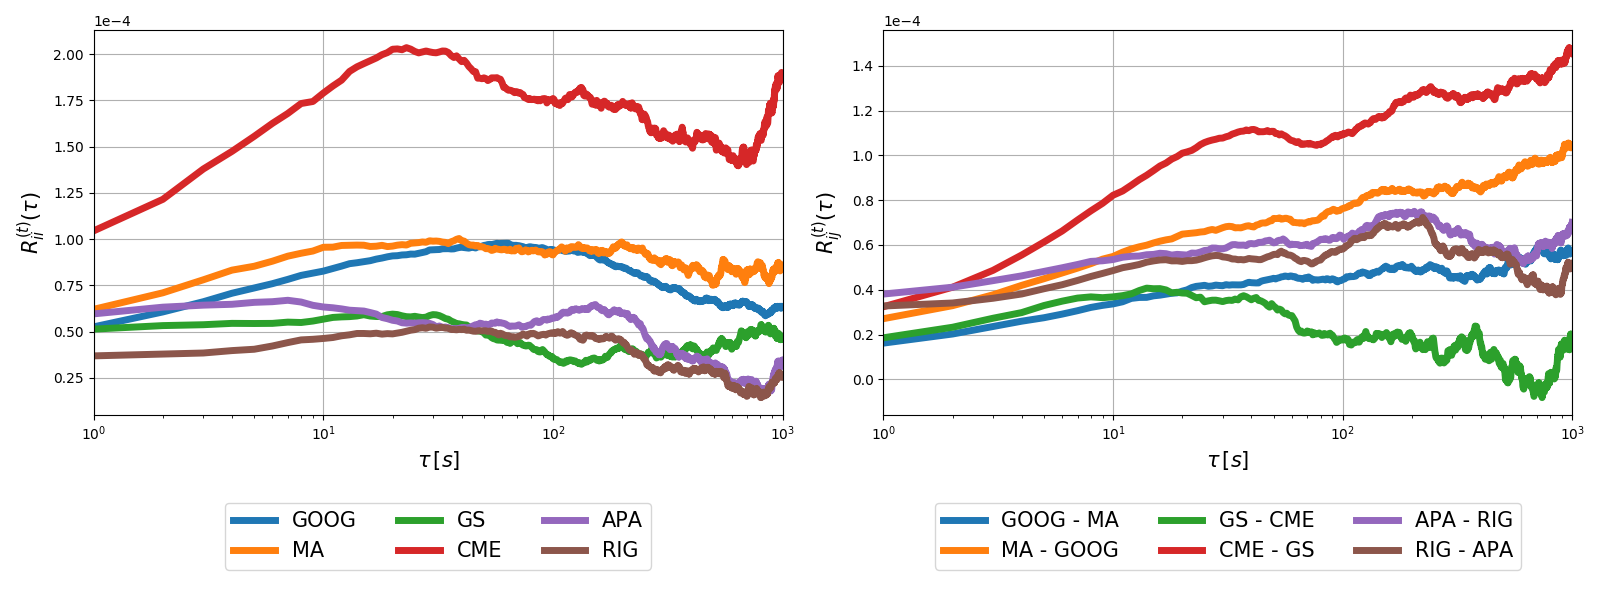
\includegraphics[width=\textwidth]
    {figures/03_responses_trade_scale_2008.png}
    \caption{Self- and cross-response functions
             $R^{\left(t\right)}_{ij}\left(\tau\right)$ in 2008 versus time lag
             $\tau$ on a logarithmic scale in trade time scale. Self-response
             functions (left) of individual stocks and cross-response functions
             (right) of stock pairs from the same economic sector.}
    \label{fig:response_function_trade_scale}
\end{figure*}

The results of Fig. \ref{fig:response_function_trade_scale} show the self-
responses of the six stocks used in the analysis and the cross-responses for
pairs of stocks representing three different economic sectors.

The self-response functions increase to a maximum and then slowly decrease. In
some stocks this behavior is more pronounced than in others. For our selected
tickers, a time lag of $\tau = 10^{3}s$ is enough to see an increase to a
maximum followed by a decrease. Thus, the trend in the self-response functions
is eventually reversed.
On the other hand, the cross-response functions have smaller signal strength
than the self-response functions. For our cross-response functions of stocks in
the same sectors, some couples exhibit the increase-decrease behavior inside a
time lag of $\tau = 10^{3}s$. Other couples seems to need a larger time lag to
reach the decrease behavior.

%%%%%%%%%%%%%%%%%%%%%%%%%%%%%%%%%%%%%%%%%%%%%%%%%%%%%%%%%%%%%%%%%%%%%%%%%%%%%%%
\subsection{Response functions on physical time scale}
\label{subsec:response_function_physical}

One important detail to compute the market response in physical time scale is
to define how the averaging of the function will be made, because the
response functions highly differ when we include or exclude
$\varepsilon^{\left(p\right)}_j \left( t\right) = 0$ \cite{Wang_2016_cross}.
The price responses including
$\varepsilon^{\left(p\right)}_j \left( t\right) = 0$ are weaker than the
excluding ones due to the omission of direct influence of the lack of trades.
However, either including or excluding $\varepsilon^{p}_j \left( t\right) = 0$
does not change the trend of price reversion versus the time lag, but it does
affect the response function strength \cite{Wang_2016_avg}. For a deeper
analysis of the influence of the term
$\varepsilon^{\left(p\right)}_j \left( t\right) = 0$, we suggest to check Refs.
\cite{Wang_2016_avg,Wang_2016_cross}. We will only take in account the
response functions excluding $\varepsilon^{p}_j \left( t\right) = 0$.

We define the self- and cross-response functions in physical time scale, using
the trade signs and the returns in physical time scale. The price response
function on physical time scale is defined as
\begin{equation}\label{eq:response_functions_time_scale_general}
    R^{\left(p\right)}_{ij}\left(\tau\right)=\left\langle r^{\left(p\right)}
    _{i}\left(t-1, \tau\right) \varepsilon_{j}^{\left(p\right)} \left(t\right)
    \right\rangle _{P}
\end{equation}
where the superscript $p$ refers to the physical time scale. The explicit
expression corresponding to Eq.
(\ref{eq:response_functions_time_scale_general}) reads
\begin{align}\label{eq:response_seconds_explicit}
    R_{ij}^{\left(p\right)}\left(\tau\right)&=\frac{1}{\sum_{d=d_{0}}^{d_{f}}
    \sum_{t=t_{0}}^{t_{f}} \eta\left[ \varepsilon_{j,d}^{\left(p\right)}
    \left(t\right)\right]} \nonumber \\
    &\sum_{d=d_{0}}^{d_{f}} \sum_{t=t_{0}}^{t_{f}}
    r^{\left(p\right)}_{i,d}\left(t-1,\tau\right)
    \varepsilon_{j,d}^{\left(p\right)}\left(t\right)
    \eta\left[\varepsilon_{j}^{\left(p\right)} \left(t\right)\right] \\
    &=\sum_{d=d_{0}}^{d_{f}}\sum_{t=t_{0}}^{t_{f}}r^{\left(p\right)}_{i,d}
    \left(t-1,\tau\right) \frac{\varepsilon_{j,d}^{\left(p\right)}
    \left(t\right) \eta\left[\varepsilon_{j,d}^{\left(p\right)}
    \left( t\right)\right]} {\sum_{d=d_{0}}^{d_{f}}\sum_{t=t_{0}}^{t_{f}}\eta
    \left[\varepsilon_{j,d}^{\left(p\right)} \left(t\right)\right]} \nonumber\\
    &=\sum_{d=d_{0}}^{d_{f}}\sum_{t=t_{0}}^{t_{f}}r^{\left(p\right)}_{i,d}
    \left(t-1,\tau\right) \text{sgn}\left(E_{j,d}\left(t\right)\right)
    w_{j,d}^{\left(p\right)}\left(t\right)
\end{align}
where
\begin{equation}
    \eta\left(x\right)=\left\{ \begin{array}{cc}
    1, & \text{If }x\ne0 \\
    0, & \text{otherwise}
    \end{array}\right.
\end{equation}

take only in account the seconds with trades and
\begin{equation}
    w_{j,d}^{\left(p\right)}\left(t\right) = \frac{\eta\left[\text{sgn}
    \left(E_{j,d}\left( t\right)\right)\right]}{\sum_{d=d_{0}}^{d_{f}}
    \sum_{t=t_{0}}^{t_{f}} \eta\left[\text{sgn}\left(E_{j,d}
    \left(t\right)\right)\right]}
\end{equation}

is a weight function that depends on the normalization of the response.

\begin{figure*}[htbp]
    \centering
    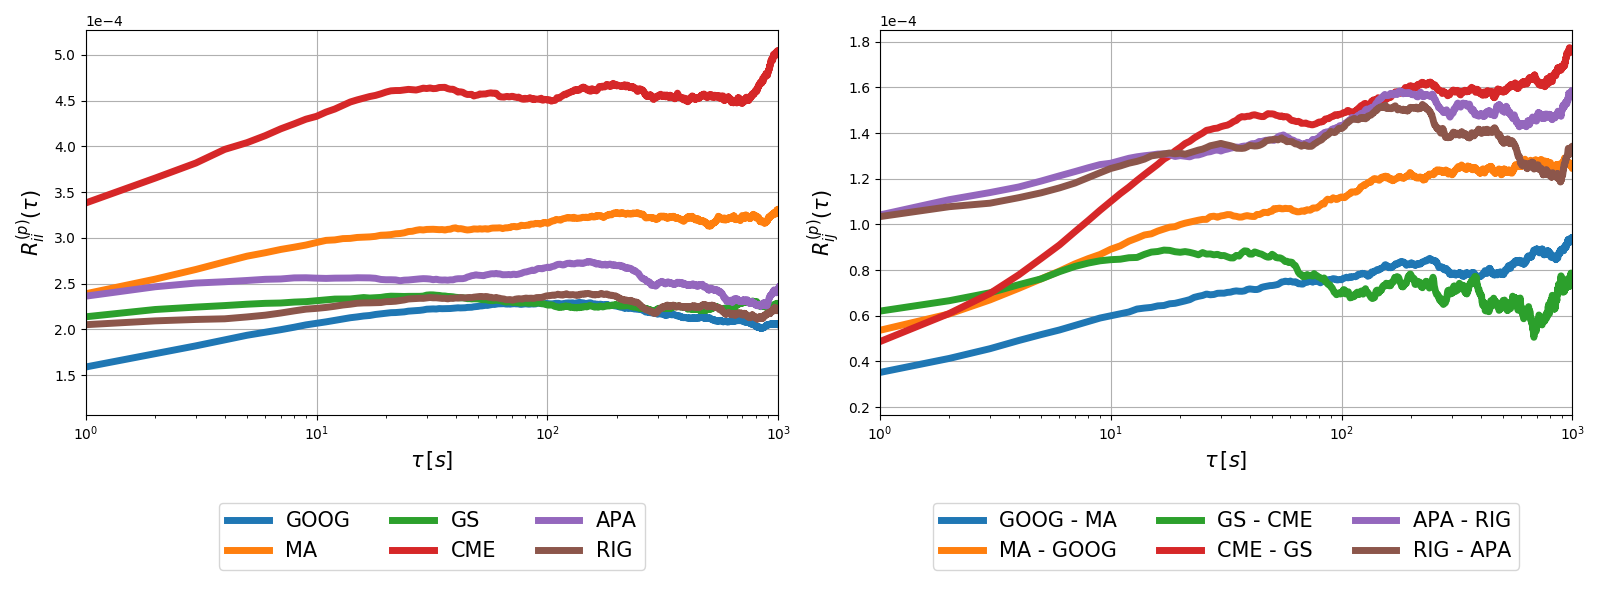
\includegraphics[width=\textwidth]
    {figures/03_responses_physical_scale_2008.png}
    \caption{Self- and cross-response functions
             $R^{\left(p\right)}_{ij}\left(\tau\right)$ excluding
             $\varepsilon^{\left(p\right)}_{j}\left(t\right) = 0$ in 2008
             versus time lag $\tau$ on a logarithmic scale in physical time
             scale. Self-response functions (left) of individual stocks and
             cross-response functions (right) of stock pairs from the same
             economic sector.}
    \label{fig:market_response_time_scale}
\end{figure*}

The results showed in Fig. \ref{fig:market_response_time_scale} are the
self- and cross-response functions in physical time scale. For the
self-response functions we can say again that in almost all the cases, an
increase to a maximum is followed by a decrease. Thus, the trend in the self-
and cross-response is eventually reversed.
In the cross-response functions, we have a similar behavior with the previous
subsection, where the time lag in some pairs was not enough to see the decrease
of the response.

Compared with the response functions in trade time scale, the response functions
in physical time scale are stronger.

%%%%%%%%%%%%%%%%%%%%%%%%%%%%%%%%%%%%%%%%%%%%%%%%%%%%%%%%%%%%%%%%%%%%%%%%%%%%%%%
\subsection{Activity response functions on physical time scale}
\label{subsec:activity_response_function}

Finally, we define the activity self- and cross-response functions in physical
time scale, using the trade signs and the returns in physical time scale.
We add a factor $N_{j,d} \left(t \right)$ to check the influence of the
frequency of trades in a second in the response functions. The activity price
response function is defined as

\begin{equation}\label{eq:activity_response_functions_general}
    R^{\left(p, a\right)}_{ij}\left(\tau\right)=\left\langle r^{\left(p\right)}
    _{i}\left(t-1, \tau\right) \varepsilon_{j}^{\left(p\right)} \left(t\right)
    N \left(t \right) \right\rangle _{P}
\end{equation}

where the superscript $a$ refers to the activity response function. The
corresponding explicit expression reads

\begin{align}
    R_{ij}^{\left(p, a\right)}\left(\tau\right)&=\frac{1}{\sum_{d=d_{0}}
    ^{d_{f}} \sum_{t=t_{0}}^{t_{f}}N_{j,d} \left(t\right)} \nonumber \\
    &\sum_{d=d_{0}}^{d_{f}}\sum_{t=t_{0}}^{t_{f}}r^{\left(p\right)}_{i,d}
    \left(t-1,\tau\right) \varepsilon_{j,d}^{\left(p\right)}\left(t\right)
    N_{j,d} \left(t\right)\\
    &=\sum_{d=d_{0}}^{d_{f}} \sum_{t=t_{0}}^{t_{f}}r^{\left(p\right)}_{i,d}
    \left(t-1,\tau\right) \frac{\varepsilon_{j,d}^{\left(p\right)}\left(t \right)
    N_{j,d}\left(t\right)} {\sum_{d=d_{0}}^{d_{f}}\sum_{t=t_{0}}^{t_{f}}
    N_{j,d}\left(t \right)} \nonumber \\
    &=\sum_{d=d_{0}}^{d_{f}} \sum_{t=t_{0}}^{t_{f}}r^{\left(p\right)}_{i,d}
    \left(t-1,\tau\right) \text{sgn}\left(E_{j,d}\left(t\right)\right)
    w_{j,d}^{\left(a\right)}\left(t\right)
\end{align}
where
\begin{equation}
    w_{j,d}^{\left(a\right)}\left(t\right) = \frac{N_{j,d}\left(t \right)}
    {\sum_{d=d_{0}}^{d_{f}}\sum_{t=t_{0}}^{t_{f}}N_{j,d}\left(t\right)}
\end{equation}
is a weight function that depends on the normalization of the response.

As $E_{j,d}\left(t\right)$ is the sum of $+1$ and $-1$ in one second and
$N_{j,d}\left(t\right)$ is the number of trades in a second,
$N_{j,d}\left(t\right) \ge E_{j,d}\left(t\right)$.
$N_{j,d}\left(t\right) = E_{j,d}\left(t\right)$ only when all the trades in a
second are buys $(+1)$.

The trade weight $w_{j,d}^{\left(t\right)}\left(t\right)$ reduces noises, The
physical weight $w_{j,d}^{\left(p\right)}\left(t\right)$ gives every step the
same weight, and the activity weight $w_{j,d}^{\left(a\right)}\left(t\right)$
emphasizes seconds with large activity.

In Fig. \ref{fig:relation_responses}, we can see how the three
responses have approximately the same shape, but the strength of the signal
varies depending on the definition. The frequency of trades have a large
influence in the responses.

\begin{figure*}[htbp]
    \centering
    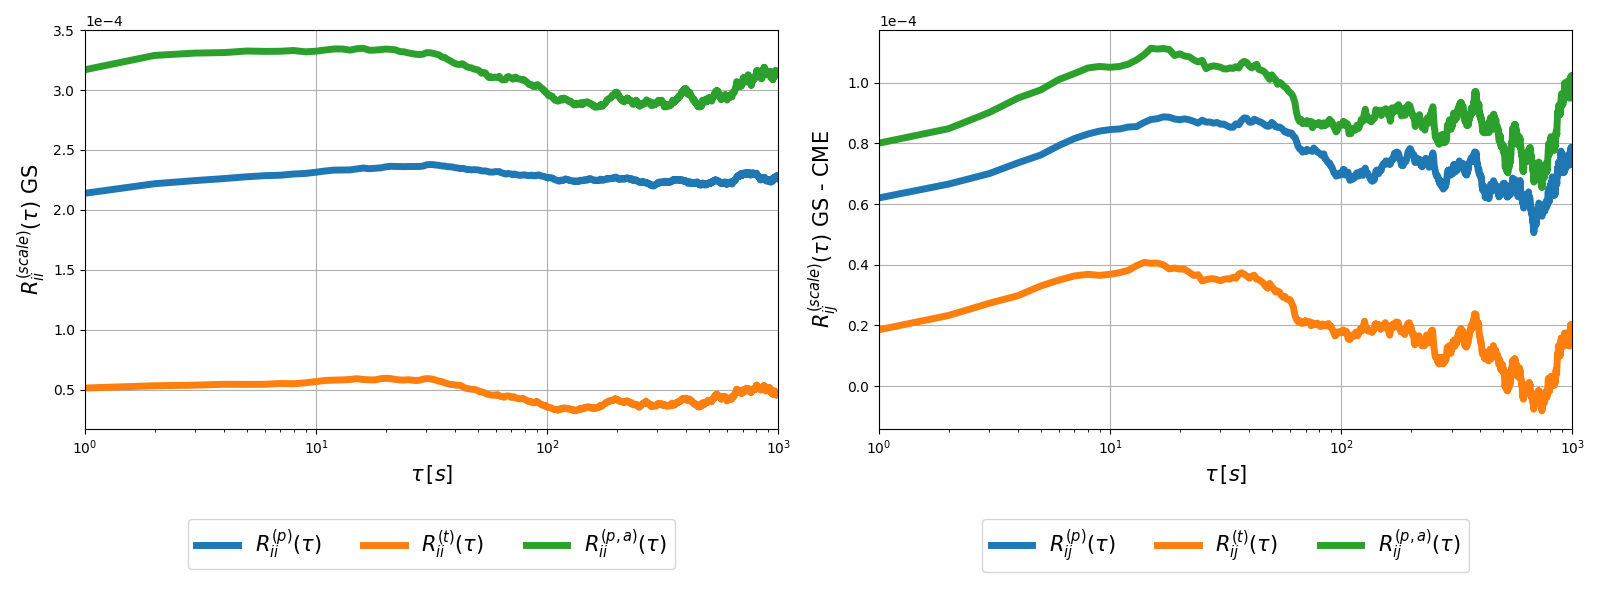
\includegraphics[width=\textwidth]
    {figures/03_response_comparison_2008_GSi_CMEj.png}
    \caption{Self- and cross-response functions
             $R^{\left(scale\right)}_{ij}\left(\tau\right)$ excluding
             $\varepsilon^{\left(p\right)}_{j}\left(t\right) = 0$ in 2008
             versus time lag $\tau$ on a logarithmic scale. Self-response
             functions (left) of Goldman Sachs Group Inc. stock and
             cross-response functions (right) of Goldman Sachs Group Inc.-CME
             Group Inc. stocks.}
    \label{fig:relation_responses}
\end{figure*}

As predicted by the weights, the event response is weaker than the physical
response, and the activity response is the strongest response.

We propose a methodology to directly compare price response functions in trade
time scale and physical time scale. Additionally, we suggest a new definition
to measure the impact of the number of trades in physical time scale. In the
three curves in the figure can be seen the increase-decrease behavior of the
response functions.

Our results are consistent with the current literature, where the results
differ about a factor of two depending on the time scale. We note that the
activity response function implementation is only a test and was never defined
in previous works. That is why the difference of a factor of two can not be
seen in Fig. \ref{fig:relation_responses} for
$R_{ij}^{\left(p,a\right)} \left( \tau \right)$.

